\subsection{Simulação para todo o ano de 2021}
\label{section: sim-2021}
Foi criado um modelo para simular todo o ano de 2021 e os diferentes intervalos entre chegadas ao longo do ano utilizando a lógica da programação dos intervalos de chegadas presentes na Figura \ref*{fig: logica-2021}. Conforme a simulação avança, a média da geração de número aleatórios conforme distribuição exponencial diminui.

\begin{figure}[H]
    \centering
    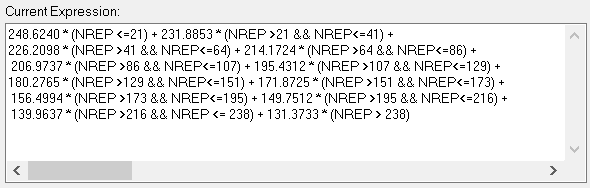
\includegraphics[scale=1.2]{simulacao/logica-2021.png}
    \caption{Programação dos intervalos entre chegadas ao longo de 2021}
    \label{fig: logica-2021}
\end{figure}

O arquivo obtido dessa simulação foi validado, mês a mês, com os dados históricos. A Figura \ref*{fig: validacao-sim-2021} mostra que nenhuma hipótese nula para o teste de Kolmogorov Smirnov de 2 amostras foi rejeitada, o que significa que a simulação dia a dia é uma boa representante do sistema real ao analisarmos os tempos relevantes para o sistema. A partir desta validação, é possível realizar a simulação dia a dia para o ano seguinte, permitindo planejar novas estratégias de gestão que auxiliem no cumprimento da meta de atendimento da empresa.

\begin{figure}[H]
    \centering
    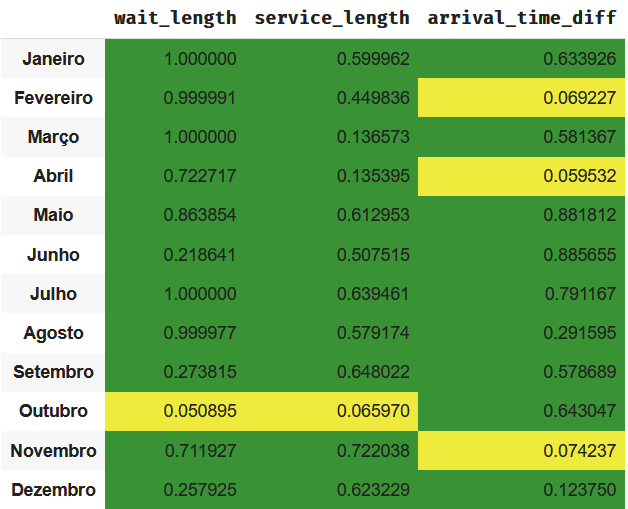
\includegraphics[scale=1]{simulacao/validacao-sim-2021.png}
    \caption{Teste de hipóteses para a simulação do ano de 2021 mês a mês}
    \label{fig: validacao-sim-2021}
\end{figure}
